\documentclass{classrep}
\usepackage{color}
\usepackage{url}
\usepackage{hyperref}
\usepackage{amsmath}
\usepackage[T1]{fontenc}
\usepackage{polski}
\usepackage[utf8]{inputenc}
\usepackage{graphicx}
\graphicspath{ {./rys/} }

\usepackage{etoolbox}
\let\bbordermatrix\bordermatrix
\patchcmd{\bbordermatrix}{8.75}{4.75}{}{}
\patchcmd{\bbordermatrix}{\left(}{\left[}{}{}
\patchcmd{\bbordermatrix}{\right)}{\right]}{}{}

\studycycle{Informatyka, studia dzienne, I st.}
\coursesemester{VI}

\coursename{Komputerowe systemy rozpoznawania}
\courseyear{2019/2020}

\courseteacher{dr inż. Marcin Kacprowicz}
\coursegroup{poniedziałek, 12:00}

\author{
	\studentinfo{Radosław Grela}{216769} \and
	\studentinfo{Jakub Wąchała}{216914} 
}

\title{Zadanie 2: Lingwistyczne podsumowania baz danych}


\begin{document}
	\maketitle
	
	\section{Cel} % Cel
	
	
	\section{Wprowadzenie} % Wprowadzenie
	
	\subsection{Funkcja trapezoidalna}
	Funkcja trapezoidalna przyjmuje 4 parametry a, b, c, d, dla których spełniony jest warunek a $\leq$ b $\leq$ c $\leq$ d. Jej wzór jest następujący \cite{anbook}: 
	
	\begin{equation}
	\mu_A(x) = \begin{cases}
	\frac{x-a}{b-a} & \mbox{gdy } x \in (a,\, b), \\
	1                 & \mbox{gdy } x \in [b,\, c], \\
	\frac{d-x}{d-c} & \mbox{gdy } x \in (c,\, d), \\
	0                 & \mbox{w przeciwnym razie}.
	\end{cases}
	\end{equation}
	
	
	\subsection{Funkcja trójkątna}
	Funkcja trójkątna jest szczególnym przypadkiem funkcji trapezoidalnej. Przyjmuje ona trzy parametry a, b, c, dla których zachodzi warunek a $\leq$ b $\leq$ c. Te parametry określają punkty ,,załamania'' tej funkcji. Jej wzór jest następujący \cite{funkcje}: 
	\begin{equation}
	\mu_A(x) = \begin{cases}
	\frac{x-a}{b-a} & \mbox{gdy } x \in (a,\, b), \\
	1                 & \mbox{gdy } x = b, \\
	\frac{c-x}{c-b} & \mbox{gdy } x \in (b,\, c), \\
	0                 & \mbox{w przeciwnym razie}.
	\end{cases}
	\end{equation}
	
	
	
	
	\subsection{Funkcja Gaussowska} 
	Funkcja Gaussowska jest definiowana przez 2 parametry które określają środek funkcji oraz jej szerokość. Wzór jest następujący \cite{kul}:
	\begin{equation}
		\mu_A(x) = e^{(-(\frac{x - \bar{x}}{\sigma})^2)}
	\end{equation}
	gdzie 
	\begin{itemize}
		\item $\bar{x}$ jest środkiem funkcji,
		\item $\sigma$ określa szerokość krzywej Gaussowskiej. 
	\end{itemize}

	\newpage
	\section{Opis implementacji} % Opis implementacji
	Program został stworzony w języku C\#. Graficzny interfejs użytkownika został stworzony przy wykorzystaniu Windows Presentation Foundation. W programie wykorzystaliśmy bibliotekę AForge. Poniżej przedstawiamy uproszczony diagram UML naszego programu.
	
	\begin{figure}[h!]
		\centering
		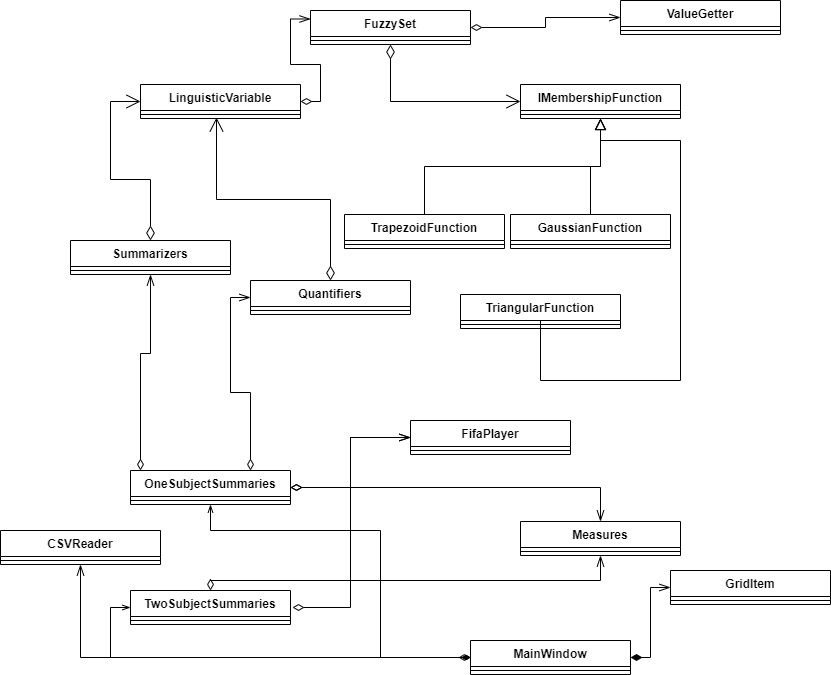
\includegraphics[width=0.9\textwidth]{../uml/uml.png}
		\caption{Diagram UML.}
		\label{uml}
	\end{figure}
	
	\begin{itemize}
		\item Klasa Summarizers odpowiada za poszczególne sumaryzatory, np "młody", "wysoki" 
		\item CSVReader odpowiada za wczytanie pliku csv z danymi do programu
		\item FifaDatabase odpowiada za bazę danych, czyli przechowywanie wszystkich rekordów
		\item FuzzySet to klasa odpowiadająca za zbiór rozmyty
		\item Klasy TrapezoidFunction, GaussianFunction, TriangularFunction odpowiadają za odpowiednie funkcje przynależności
		\item FifaPlayer to klasa, która reprezentuje krotkę bazy danych
		\item Quantifiers jest klasą odpowiedzialną za kwantyfikatory
		\item LinguisticVariable to klasa reprezentująca zmienną lingwistyczną.
	\end{itemize}
	
	\section{Materiały i metody} % Materiały i metody
	\subsection{Baza danych}
	Do przeprowadzania badań oraz do generowania podsumowań wykorzystaliśmy bazę danych dotyczącą piłkarzy z gry FIFA 20. Pochodzi ona ze źródła \cite{baza}. Składa się ona z 18278 rekordów posiadających 104 atrybuty. Do naszego projektu skorzystamy z 11. Są to następujące atrybuty:
	
	\begin{enumerate}
		\item Wiek - \textsl{age} - wartość z przedziału [16, 42]
		\item Wzrost (w cm) - \textsl{height\_cm} - wartość z przedziału [156, 205]
		\item Waga (w kg) - \textsl{weight\_kg} - wartość z przedziału [50, 110]
		\item Ocena ogólna - \textsl{overall} - wartość z przedziału [48, 94]
		\item Wykończenie - \textsl{attacking\_finishing} - wartość z przedziału [2, 95]
		\item Dribbling - \textsl{skill\_dribbling} - wartość z przedziału [4, 97]
		\item Podkręcenie piłki - \textsl{skill\_curve} - wartość z przedziału [6, 94]
		\item Długie podania - \textsl{skill\_long\_passing} - wartość z przedziału [8, 92]
		\item Sprint - \textsl{movement\_sprint\_speed} - wartość z przedziału [11, 96]
		\item Siła strzału - \textsl{power\_shot\_power} - wartość z przedziału [14, 95]
	\end{enumerate}

	Każda z kolumn jest typu całkowitego.

	\subsection{Zmienne lingwistyczne}
	% wiek -------------------------------
	\subsubsection{Wiek}
	Należy zauważyć, że wiek w przypadku zawodnika piłki nożnej oceniany jest w inny sposób niż wiek przeciętnego człowieka.
	\begin{itemize}
		\item \textsl{(16-21) bardzo młody}
		\item \textsl{(20-25) młody}
		\item \textsl{(24-32) średni}
		\item \textsl{(31-42) stary}
	\end{itemize}
	
	\begin{table}[h!]
		\centering
		\begin{tabular} {c c c c c}
			\hline
			\textbf{Etykieta} & \textbf{a} & \textbf{b} & \textbf{c} & \textbf{d} \\ [0.5ex] 
			\hline	
			\hline 
			bardzo młody & 16 & 16 & 18 & 21  \\
			młody & 20 & 22 & 24 & 25  \\
			średni & 24 & 26 & 29 & 32  \\
			stary & 31 & 34 & 42 & 42  \\
			\hline
		\end{tabular}
		\caption{Przyporządkowane parametry funkcji trapezoidalnej dla atrybutu  Wiek. }
		\label{tabelaWiek}
	\end{table}

	\begin{figure}[h!]
		\centering
		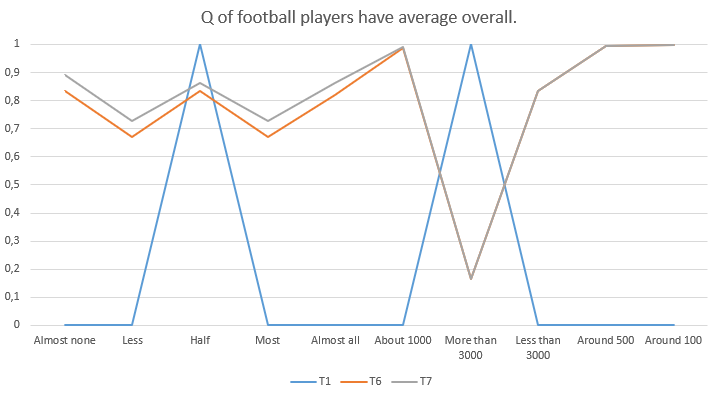
\includegraphics[width=0.9\textwidth]{zmienne/1.png}
		\caption{Funkcja przynależności (trapezoidalna) dla atrybutu Wiek.}
		\label{wykresWiek}
	\end{figure}
	
	% wzrost ---------------------------
	\newpage
	\subsubsection{Wzrost}
	\begin{itemize}
		\item \textsl{(156-166) niski}
		\item \textsl{(164-177) średni}
		\item \textsl{(175-188) wysoki}
		\item \textsl{(186-205) bardzo wysoki}
	\end{itemize}
	
	\begin{table}[h!]
		\centering
		\begin{tabular} {c c c c}
			\hline
			\textbf{Etykieta} & \textbf{a} & \textbf{b} & \textbf{c} \\ [0.5ex] 
			\hline	
			\hline 
			niski & 156 & 156 & 166 \\
			średni & 164 & 170 & 177 \\
			wysoki & 175 & 182 & 188 \\
			bardzo wysoki & 186 & 205 & 205  \\
			\hline
		\end{tabular}
		\caption{Przyporządkowane parametry funkcji trójkątnej dla atrybutu Wzrost. }
		\label{tabelaWzrost}
	\end{table}
	
	\begin{figure}[h!]
		\centering
		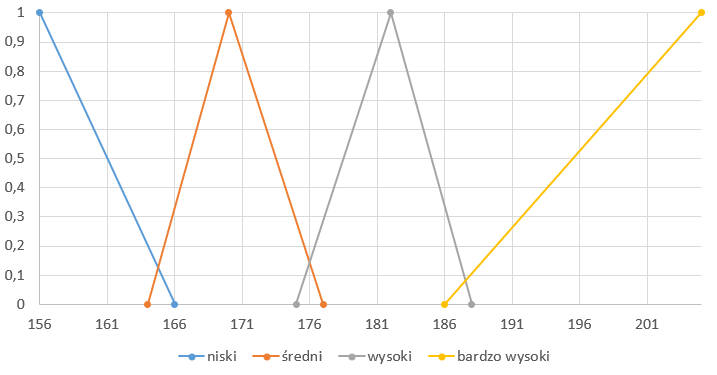
\includegraphics[width=0.9\textwidth]{zmienne/2.png}
		\caption{Funkcja przynależności (trapezoidalna) dla atrybutu Wzrost.}
		\label{wykresWzrost}
	\end{figure}

	% waga ---------------------------
	\newpage
	\subsubsection{Waga}
	\begin{itemize}
		\item \textsl{(50-65) bardzo chudy}
		\item \textsl{(55-85) chudy}
		\item \textsl{(75-105) średni}
		\item \textsl{(95-110) gruby}
	\end{itemize}
	
	\begin{table}[h!]
		\centering
		\begin{tabular} {c c c}
			\hline
			\textbf{Etykieta} & \textbf{$\bar{x}$} & \textbf{$\sigma$} \\ [0.5ex] 
			\hline	
			\hline 
			bardzo chudy & 50 & 8  \\
			chudy & 70 & 8  \\
			średni & 90 & 8  \\
			gruby & 110 & 8  \\
			\hline
		\end{tabular}
		\caption{Przyporządkowane parametry funkcji gaussowskiej dla atrybutu  Waga. }
		\label{tabelaWaga}
	\end{table}
	
	\begin{figure}[h!]
		\centering
		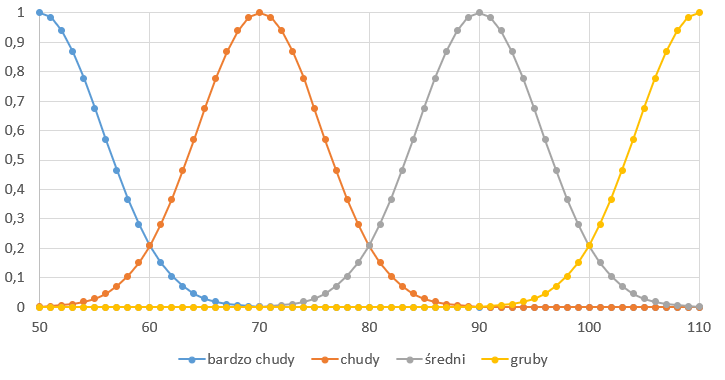
\includegraphics[width=0.9\textwidth]{zmienne/3.png}
		\caption{Funkcja przynależności (gaussowska) dla atrybutu Waga.}
		\label{wykresWaga}
	\end{figure}
	
	% Ocena ogólna -------------------------------
	\newpage
	\subsubsection{Ocena ogólna}
	\begin{itemize}
		\item \textsl{(48-65) słaby}
		\item \textsl{(60-75) średni}
		\item \textsl{(70-87) dobry}
		\item \textsl{(85-94) bardzo dobry}
	\end{itemize}
	
	\begin{table}[h!]
		\centering
		\begin{tabular} {c c c c c}
			\hline
			\textbf{Etykieta} & \textbf{a} & \textbf{b} & \textbf{c} & \textbf{d} \\ [0.5ex] 
			\hline	
			\hline 
			słaby & 48 & 48 & 59 & 65  \\
			średni & 60 & 65 & 70 & 75  \\
			dobry & 70 & 78 & 85 & 87  \\
			bardzo dobry & 85 & 90 & 94 & 94  \\
			\hline
		\end{tabular}
		\caption{Przyporządkowane parametry funkcji trapezoidalnej dla atrybutu  Ocena ogólna. }
		\label{tabelaOverall}
	\end{table}
	
	\begin{figure}[h!]
		\centering
		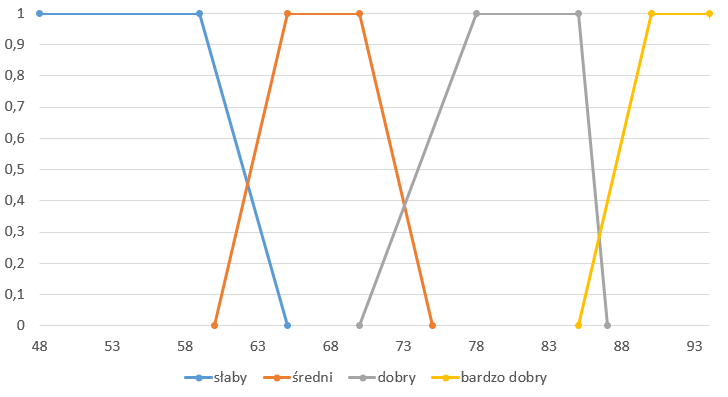
\includegraphics[width=0.9\textwidth]{zmienne/4.png}
		\caption{Funkcja przynależności (trapezoidalna) dla atrybutu Ocena ogólna.}
		\label{wykresOverall}
	\end{figure}
	
	
	% Wykończenie -------------------------------
	\newpage
	\subsubsection{Wykończenie}
	\begin{itemize}
		\item \textsl{(2-35) bardzo słabe}
		\item \textsl{(30-60) słabe}
		\item \textsl{(50-80) średnie}
		\item \textsl{(75-87) dobre}
		\item \textsl{(85-95) bardzo dobre}
	\end{itemize}
	
	\begin{table}[h!]
		\centering
		\begin{tabular} {c c c c c}
			\hline
			\textbf{Etykieta} & \textbf{a} & \textbf{b} & \textbf{c} & \textbf{d} \\ [0.5ex] 
			\hline	
			\hline 
			bardzo słabe & 2 & 2 & 25 & 35  \\
			słabe & 30 & 35 & 50 & 60  \\
			średnie & 50 & 55 & 75 & 80  \\
			dobre & 75 & 80 & 85 & 87  \\
			bardzo dobre & 85 & 90 & 95 & 95  \\			
			\hline
		\end{tabular}
		\caption{Przyporządkowane parametry funkcji trapezoidalnej dla atrybutu  Wykończenie. }
		\label{tabelaWykonczenie}
	\end{table}
	
	\begin{figure}[h!]
		\centering
		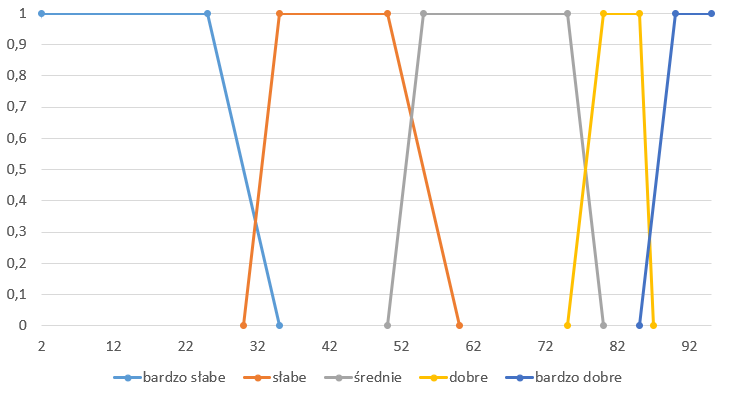
\includegraphics[width=0.9\textwidth]{zmienne/5.png}
		\caption{Funkcja przynależności (trapezoidalna) dla atrybutu Wykończenie.}
		\label{wykresWykonczenie}
	\end{figure}

	
	% Dribbling -------------------------------
	\newpage
	\subsubsection{Dribbling}
	\begin{itemize}
		\item \textsl{(4-35) bardzo słaby}
		\item \textsl{(30-60) słaby}
		\item \textsl{(50-70) średni}
		\item \textsl{(68-87) dobry}
		\item \textsl{(85-97) bardzo dobry}
	\end{itemize}
	
	\begin{table}[h!]
		\centering
		\begin{tabular} {c c c c c}
			\hline
			\textbf{Etykieta} & \textbf{a} & \textbf{b} & \textbf{c} & \textbf{d} \\ [0.5ex] 
			\hline	
			\hline 
			bardzo słaby & 4 & 4 & 25 &	35 \\
			słaby & 30 & 35 & 50 & 60  \\
			średni & 50 & 55 & 68 & 70  \\
			dobry & 68 & 73 & 85 & 87  \\
			bardzo dobry & 85 & 90 & 97 & 97  \\		
			\hline
		\end{tabular}
		\caption{Przyporządkowane parametry funkcji trapezoidalnej dla atrybutu Dribbling. }
		\label{tabelaDribbling}
	\end{table}
	
	\begin{figure}[h!]
		\centering
		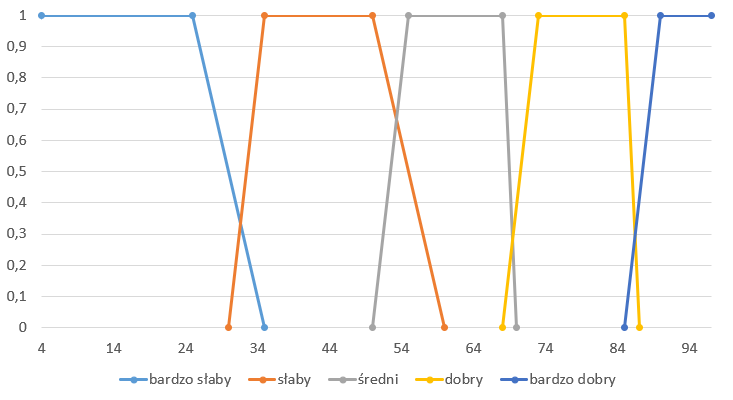
\includegraphics[width=0.9\textwidth]{zmienne/6.png}
		\caption{Funkcja przynależności (trapezoidalna) dla atrybutu Dribbling.}
		\label{wykresDribbling}
	\end{figure}
	
	
	% Podkręcenie piłki -------------------------------
	\newpage
	\subsubsection{Podkręcenie piłki}
	\begin{itemize}
		\item \textsl{(6-35) bardzo słabe}
		\item \textsl{(30-60) słabe}
		\item \textsl{(50-70) średnie}
		\item \textsl{(68-87) dobre}
		\item \textsl{(85-94) bardzo dobre}
	\end{itemize}
	
	\begin{table}[h!]
		\centering
		\begin{tabular} {c c c c}
			\hline
			\textbf{Etykieta} & \textbf{a} & \textbf{b} & \textbf{c} \\ [0.5ex] 
			\hline	
			\hline 
			bardzo słabe & 6 & 6 & 35 \\
			słabe & 20 & 35 & 60   \\
			średnie & 50 & 60 & 70  \\
			dobre & 68 & 75 & 87   \\
			bardzo dobre & 85 & 94 & 94  \\					
			\hline
		\end{tabular}
		\caption{Przyporządkowane parametry funkcji trójkątnej dla atrybutu Podkręcenie piłki. }
		\label{tabelaPodkrecenie}
	\end{table}
	
	\begin{figure}[h!]
		\centering
		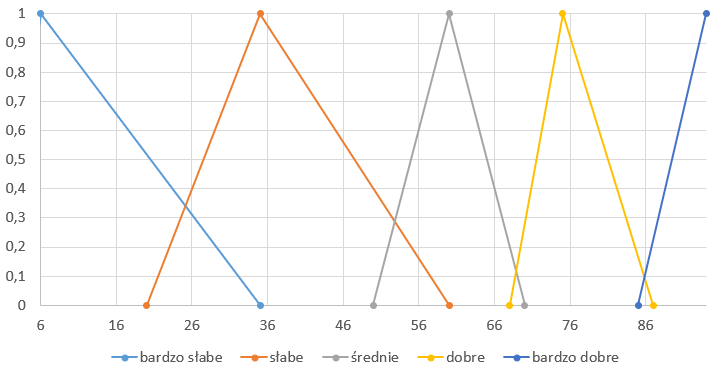
\includegraphics[width=0.9\textwidth]{zmienne/7.png}
		\caption{Funkcja przynależności (trójkątna) dla atrybutu Podkręcenie piłki.}
		\label{wykresPodkrecenie}
	\end{figure}
	
	
	% Długie podania -------------------------------
	\newpage
	\subsubsection{Długie podania}
	\begin{itemize}
		\item \textsl{(8-35) bardzo słabe}
		\item \textsl{(30-60) słabe}
		\item \textsl{(50-70) średnie}
		\item \textsl{(68-85) dobre}
		\item \textsl{(82-92) bardzo dobre}
	\end{itemize}
	\begin{table}[h!]
		\centering
		\begin{tabular} {c c c c c}
			\hline
			\textbf{Etykieta} & \textbf{a} & \textbf{b} & \textbf{c} & \textbf{d} \\ [0.5ex] 
			\hline	
			\hline 
			bardzo słabe & 8 & 8 & 25 &	35 \\
			słabe & 30 & 35 & 50 & 60  \\
			średnie & 50 & 55 & 68 & 70  \\
			dobre & 68 & 73 & 80 & 85  \\
			bardzo dobre & 82 & 85 & 92 & 92  \\	
			\hline
		\end{tabular}
		\caption{Przyporządkowane parametry funkcji trapezoidalnej dla atrybutu Długie podania. }
		\label{tabelaPodania}
	\end{table}
	\begin{figure}[h!]
		\centering
		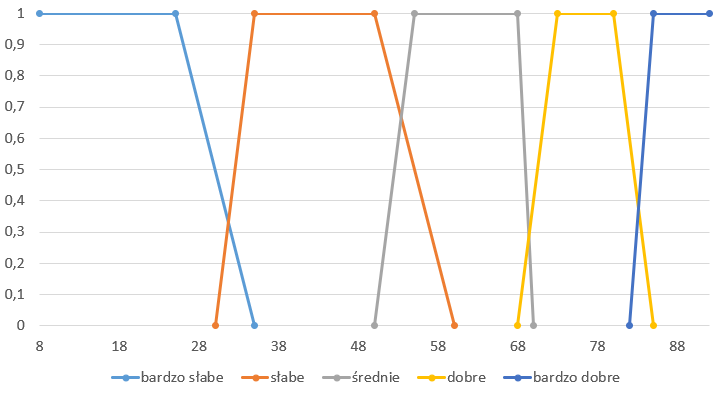
\includegraphics[width=0.9\textwidth]{zmienne/8.png}
		\caption{Funkcja przynależności (trapezoidalna) dla atrybutu Długie podania.}
		\label{wykresPodania}
	\end{figure}

	% Sprint -------------------------------
	\newpage
	\subsubsection{Sprint}
	\begin{itemize}
		\item \textsl{(11-35) bardzo wolny}
		\item \textsl{(30-55) wolny}
		\item \textsl{(50-70) średni}
		\item \textsl{(68-86) szybki}
		\item \textsl{(84-96) bardzo szybki}
	\end{itemize}
	\begin{table}[h!]
		\centering
		\begin{tabular} {c c c c c}
			\hline
			\textbf{Etykieta} & \textbf{a} & \textbf{b} & \textbf{c} & \textbf{d} \\ [0.5ex] 
			\hline	
			\hline 
			bardzo wolny & 11 & 11 & 25 &	35 \\
			wolny & 30 & 35 & 48 & 55  \\
			średni & 50 & 55 & 68 & 70  \\
			szybki & 68 & 73 & 80 & 86  \\
			bardzo szybki & 84 & 90 & 96 & 96  \\	
			\hline
		\end{tabular}
		\caption{Przyporządkowane parametry funkcji trapezoidalnej dla atrybutu Sprint. }
		\label{tabelaSprint}
	\end{table}
	\begin{figure}[h!]
		\centering
		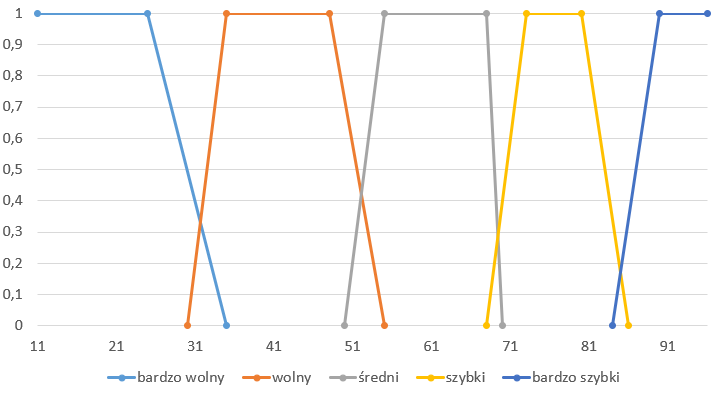
\includegraphics[width=0.9\textwidth]{zmienne/9.png}
		\caption{Funkcja przynależności (trapezoidalna) dla atrybutu Sprint.}
		\label{wykresSprint}
	\end{figure}


	% Siła strzału -------------------------------
	\newpage
	\subsubsection{Siła strzału}
	\begin{itemize}
		\item \textsl{(14-50) słaba}
		\item \textsl{(45-65) średnia}
		\item \textsl{(62-82) duża}
		\item \textsl{(80-95) bardzo duża}
	\end{itemize}
	\begin{table}[h!]
		\centering
		\begin{tabular} {c c c c c}
			\hline
			\textbf{Etykieta} & \textbf{a} & \textbf{b} & \textbf{c} & \textbf{d} \\ [0.5ex] 
			\hline	
			\hline 
			słaba & 14 & 14 & 45 & 50 \\
			średnia & 45 & 50 & 60 & 65  \\
			duża & 62 & 68 & 80 & 82  \\
			bardzo duża & 80 & 88 & 95 & 95  \\			
			\hline
		\end{tabular}
		\caption{Przyporządkowane parametry funkcji trapezoidalnej dla atrybutu Siła strzału. }
		\label{tabelaStrzal}
	\end{table}
	\begin{figure}[h!]
		\centering
		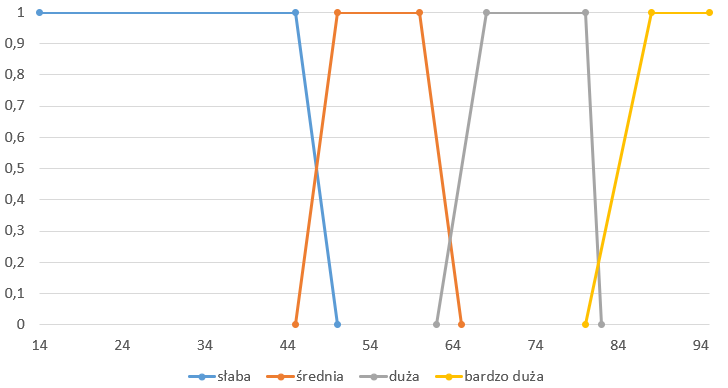
\includegraphics[width=0.9\textwidth]{zmienne/10.png}
		\caption{Funkcja przynależności (trapezoidalna) dla atrybutu Siła strzału.}
		\label{wykresStrzal}
	\end{figure}

	\newpage
	\subsection{Kwantyfikator względny}
	
	Poniżej przedstawiliśmy wartości parametrów oraz wykres funkcji przynależności dla kwantyfikatora względnego. Liczba rekordów w naszej bazie danych wynosi 18278, wykres zawiera się w wartościach [0, 1].
	\begin{table}[h!]
		\centering
		\begin{tabular} {c c c c c}
			\hline
			\textbf{Etykieta} & \textbf{a} & \textbf{b} & \textbf{c} & \textbf{d} \\ [0.5ex] 
			\hline	
			\hline 
			prawie nikt			 & 0,000 & 0,000 & 0,055 & 0,164 \\
			mniejszość			 & 0,109 & 0,164 & 0,383 & 0,438  \\
			połowa				 & 0,410 & 0,438 & 0,547 & 0,574  \\
			większość 		 	 & 0,547 & 0,602 & 0,821 & 0,875  \\	
			prawie wszyscy		 & 0,821 & 0,903 & 1,000 & 1,000  \\						
			\hline			
		\end{tabular}
		\caption{Przyporządkowane parametry funkcji trapezoidalnej dla kwantyfikatora względnego. }
		\label{tabelaKwantyfikatorWzgledny}
	\end{table}
	
	\begin{figure}[h!]
		\centering
		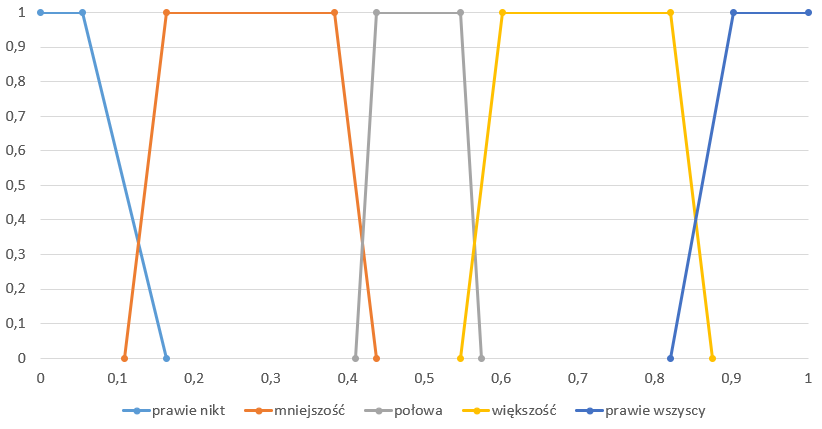
\includegraphics[width=0.9\textwidth]{kwantyfikatorWzgledny.png}
		\caption{Funkcja przynależności kwantyfikatora względnego.}
		\label{kwantyfikatorWzgledny}
	\end{figure}
	
	\newpage
	\section{Wyniki} % Wyniki
	
	Poniżej przedstawiamy przykładowe zdania podsumowaujące bazę danych wygenerowane przez nas program.
	\begin{figure}[h!]
		\centering
		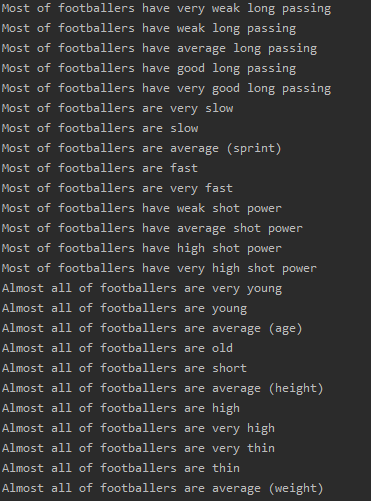
\includegraphics[width=0.9\textwidth]{zdania1.png}
		\caption{Zdania wygenerowane przez program.}
		\label{zdania}
	\end{figure}
	
	\section{Dyskusja} % Dyskusja
	
	\section{Wnioski}
		
	
	\begin{thebibliography} {0}
		\bibitem{anbook} Niewiadomski, Adam. Methods for the Linguistic Summarization of Data: Applications of Fuzzy Sets and Their Extensions. Akademicka Oficyna Wydawnicza EXIT. Warszawa, 2008. ISBN 978-83-60434-40-6
		\bibitem{baza} https://www.kaggle.com/stefanoleone992/fifa-20-complete-player-dataset 
		\bibitem{kul} https://pracownik.kul.pl/files/31717/public/Funkcje\_przynaleznosci.pdf [dostęp 07.05.2020]
		\bibitem{funkcje} http://ii.uwb.edu.pl/rudnicki/wp-content/uploads/2016/02/P07.pdf [dostęp 08.05.2020]
	\end{thebibliography}
\end{document}
